% Chapter 2
\chapter{Marco teórico} % Main chapter title

\label{Chapter2} % For referencing the chapter elsewhere, use \ref{Chapter1} 

\section{Trasfondo del aprendizaje profundo} % Main chapter title

En este capítulo se planteará y se explicará la base teórica del campo del aprendizaje profundo utilizados en este trabajo. Los conceptos descritos a continuación son el fundamento del campo de aprendizaje profundo.

El trasfondo que se compartirá en este trabajo es el fundamento teórico de las técnicas utilizadas; los fundamentos geométricos teóricos \parencite{2018leigeometric} del porqué de la funcionalidad básica de los modelos del campo no se abordarán en esta tesis.

\section{Aprendizaje supervisado}

En el área de aprendizaje (profundo) artificial existen dos tipos básicos de problema. Este se determina dependiendo de las características de los datos a utilizar para el entrenamiento del modelo \parencite{schmidhuber2015deep}.

Cuando los datos --- ya sea información tabulada, imágenes, textos --- no tienen ninguna categoría asociada o ningún valor a predecir y lo que se desea es obtener información no específica, es decir sin tener alguna referencia, se trata de un aprendizaje no supervisado.

Si los datos, por otro lado, tienen una clasificación  --- llamada etiqueta --- asignada, la cual a futuro es el resultado a predecir, los métodos a utilizar son los del \gls{aprendizaje supervisado}. Debido a que el problema a abordar en este trabajo es un problema de clasificación, el resto del fundamento teórico será basado en este tipo de contexto.

El aprendizaje supervisado puede entonces ser descrito como una función $f : X \to Y$ donde $X$ representa los datos con los que se alimenta la función, es decir las características que utilizará el modelo para inferir, y $Y$ el resultado asignado o a predecir.

Para ilustrar el proceso de aprendizaje profundo se utilizará un caso individual de la función en donde $y$ es el resultado deseado, $f(x) = \hat{y}$ es la función aplicada a un caso específico y $\hat{y}$ representa el resultado obtenido con la función el cual no necesariamente es el resultado deseado o esperado.

\textbf{El objetivo.} En concreto, buscamos una función $f$ que sea la mejor candidata para poder predecir los resultados deseados. Si definimos una función de costo $L(\hat{y}, y)$ que representa, en un valor escalar, la diferencia cuantitativa entre la evaluación de una función $f$ candidata y el resultado real $y$ podemos concluir que el objetivo es encontrar una $f^*$ que cumpla con:

\[ f^* = \min_{f \in F} \frac{1}{N} \sum_{i = 0}^{N} L(f(x_i), y_i) \]

Donde $N$ es el número de instancias de los datos para entrenar el modelo; $F$ siendo un conjunto de funciones candidatas.

\textbf{Definición de las funciones.} La base de todo modelo de aprendizaje profundo es una red neuronal --- cuyo comportamiento será definido en la siguiente sección así como otros detalles relevantes --- y su comportamiento básico puede ser descrito de la siguiente forma:

\[ f(x_i) = w x_i + b \]

Donde $x_i$ es la instancia de datos $i$ con propósitos de entreno o de predicción. Esto nos dice que $w$ y $b$ serán los parámetros a modificar de una manera sistemática para encontrar la función $f^*$. Con fines de brevedad, la concatenación de $w$ y $b$ serán representados por $\theta$.

Una posible función de pérdida en un problema de categorización para una predicción obtenida toma la forma del error de la entropía cruzada, es decir:

\[ L(\hat{y_i}, y_i) = y_i log\hat{y_i} + (1 - y_i)log(1 - \hat{y_i}) \]

Al tener la pérdida para una predicción se puede expandir esta idea para obtener la pérdida a través de un conjunto de datos, lo cual resultará muy útil cuando se deba entrenar. Para obtener una aproximación de la perdida sobre un conjunto de datos se puede utilizar el promedio sobre las perdidas individuales de los datos evaluados:

\[ L(\hat{y}, y) = - \frac{1}{N} \sum_{i = 1}^{N} [y_i log\hat{y_i} + (1 - y_i)log(1 - \hat{y_i})] \]

\textbf{Optimización de la función de costo.} Con una función a minimizar establecida y una cantidad $N$ de datos sobre los cuales se debe encontrar una función $f$ candidata cada vez mejor, se recurre al método del descenso de gradiente. Este método nos permite, utilizar propiedades básicas de las derivadas de las funciones y poco a poco avanzar hasta llegar a un valor mínimo de la función. Cada nueva función candidata entonces podrá ser derivada de la siguiente forma:

\[ f_i(x_i) = \theta_i x_i \]

Donde
\begin{equation}
\label{eq:sgdupdate}
\theta_{i + 1} = \theta_{i} - \gamma \nabla_{\theta} L(\hat{y_i}, y_i).
\end{equation}

Este proceso de utilizar el descenso de gradiente a través de las instancias nos permite  minimizar el error de la función hasta poder deducir la función que muestra el menor error, lo cual fue descrito como el objetivo principal.

\textbf{La \gls{tasa de aprendizaje}.} La velocidad de convergencia de este proceso dependerá en gran parte de $\gamma$ que representa la tasa de aprendizaje; específicamente es la ponderación que se le da al componente del gradiente cuando se propone la nueva función. Un $\gamma$ muy alto arriesga una divergencia debido a que podría oscilar alrededor de un mínimo sin nunca poder converger en él. Un $\gamma$ muy bajo, por el otro lado, puede resultar en un aprendizaje muy lento, lo cual puede llevar a un resultado no óptimo debido a limitaciones de recursos. Este concepto será importante en capítulos posteriores de este trabajo.

\section{Redes neuronales}

Las redes neuronales son el modelo base para el aprendizaje profundo. Esto debido a que ha sido demostrado que son aproximadores universales \parencite{hornik1989universal} --- es decir que para cualquier función $h$ se tiene la capacidad de encontrar un red neuronal $\hat{H}$ que aproxime a $h$ con cierto grado de precisión --- un error de $\epsilon$ --- dado que se tenga la cantidad de unidades en la red y datos suficientes para entrenar. Formalmente se dice que

\begin{equation}
\label{eq:universaltheorem}
\vert \hat{H}(x) - h(x) \vert < \epsilon
\end{equation}

Con ayuda del concepto de las redes neuronales especificaremos más acerca de la función $f$ que hasta ahora ha permanecido general, únicamente con la restricción de ser derivable. Hay diferentes tipos de redes neuronales en el campo y en este trabajo se abordarán únicamente las redes neuronales estándar y las recurrentes.

\subsection{Redes neuronales estándar}

\begin{figure}
	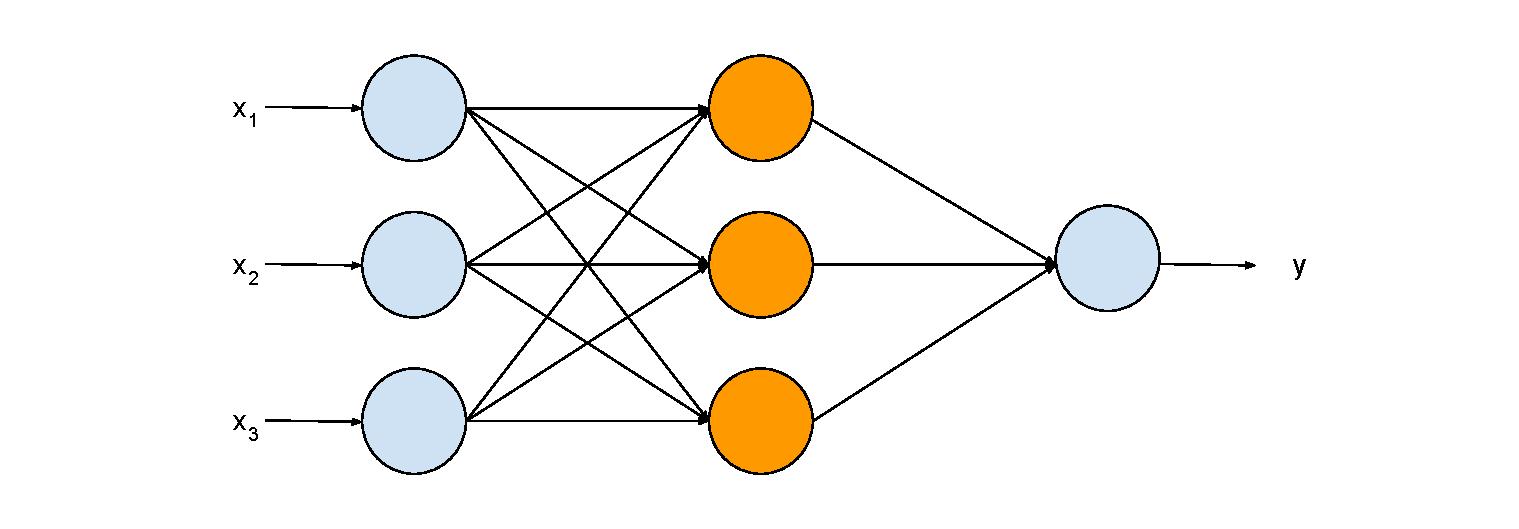
\includegraphics[scale=.6]{Figures/standardnn.pdf}
	\caption{Una red neuronal estándar con una capa oculta, la cual tiene tres unidades neuronales. La red está completamente conectada, tiene tres nodos de entrada y uno de salida.}
	\label{fig:standardnn}
\end{figure}

\textbf{Inspiración e intuición.} Estas redes neuronales fueron basadas en comportamientos biológicos y reflejan un comportamiento similar a la comunicación de neuronas que se aprecia en la naturaleza. La entrada de datos en una neurona es procesada y alimentará a la siguiente neurona y así sucesivamente hasta haber recorrido toda la red. La redes neuronales no son secuencias directas y lineales de neuronas; las redes están divididas en capas, las cuales pueden contener más de una unidad. En una red completamente conectada, como la que se aprecia en la figura \ref{fig:standardnn}, conecta a todas las unidades de una capa con todas las unidades de la siguiente. Así como las neuronas en la naturaleza, las neuronas en una red neuronal tienen una unidad o célula principal, axones y su conexión es llamada sinapsis.

\textbf{Propagación hacia adelante.} En las redes neuronales esto es el proceso del flujo de la información a través de la red, y las funciones que la componen, hasta obtener un resultado. En el caso de una red neuronal típica, este proceso significa que la salida de una neurona en una capa alimenta parcialmente a las de la capa siguiente. La función a utilizar por cada unidad individual es una regresión lineal simple que puede ser descrita como $f(x) = \mathbf{w} \mathbf{x} + b$, es decir, una matriz de parámetros a multiplicarse con los datos de entrada a la neurona. Adicional a esto se maneja una función de activación para el resultado de esa multiplicación, la cual es no lineal, a cada elemento resultante (p.e. $\tanh$). De esto se concluye que para, por ejemplo, obtener el resultado de una neurona en la cuarta capa se tiene que
\begin{equation}
\label{eq:feedfwdeq}
f(\mathbf{x}) = \mathbf{W_4} \sigma(\mathbf{W_3} \sigma (\mathbf{W_2} \sigma(\mathbf{W_1} \mathbf{x})))
\end{equation}

Donde $\mathbf{W_4}$ es una matriz de parámetros de la cuarta capa, $\mathbf{W_3}$ es una matriz de parámetros de la tercera capa, y así sucesivamente, y $\mathbf{x}$ representa los datos de entrada.

%Figura demostrando fwd y back prop
\begin{figure}
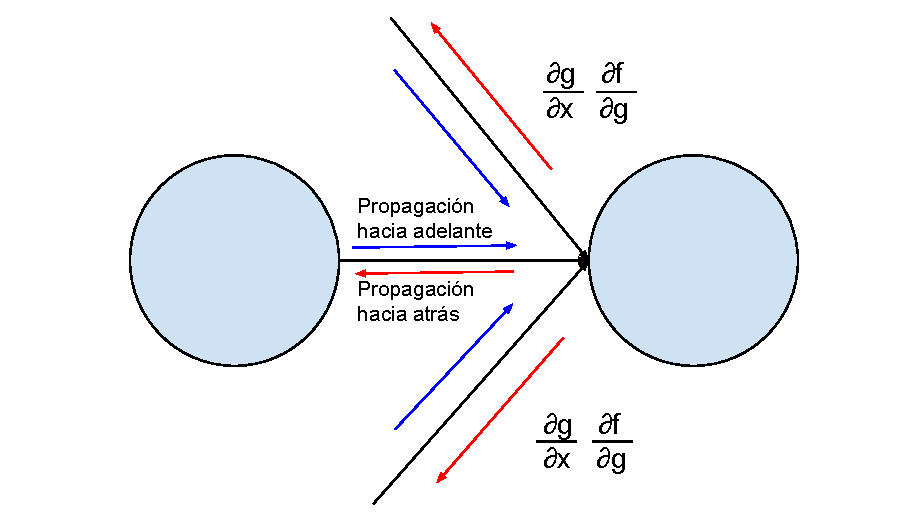
\includegraphics[scale=0.8]{Figures/backprop.pdf}
\caption{En azul se puede ver la dirección del flujo de información durante la propagación hacia adelante. En rojo se aprecia que la dirección se invierte para la propagación hacia atrás y que lleva los gradientes necesarios para propagar el error después del entrenamiento.}
\label{fig:backprop}
\end{figure}


\textbf{Propagación hacia atrás} \parencite{rumelhart1986learning}. Ya que está presente un mecanismo para evaluar el conjunto de funciones que representa cada unidad de la red, debemos tener un mecanismo para optimizar los parámetros que definen cada función. La propagación hacia atrás se encarga de esto utilizando el concepto previamente descrito como el descenso de gradiente. Para realizar la propagación hacia atrás se aplica la regla de la cadena la cual establece que $\frac{\partial f(g(x))}{\partial x} = \frac{\partial g}{\partial x} \frac{\partial f}{\partial g}$. Se debe notar que la función que se quiere derivar toma una forma similar a la que tenemos en la ecuación \ref{eq:feedfwdeq}, con la adición de que $g(x)$ es una función que anida aún más funciones. Para obtener la optimización de los parámetros podemos derivar en dirección hacia atrás propagando la mejora que se propone con el gradiente.

\subsection{Redes neuronales recurrentes}

% Figura con una LSTM y su descripcion


Este tipo de redes tienen la peculiaridad que se alimentan no solamente de los resultados de las funciones de activación de las capas anteriores sino también del resultado de la instancia previamente evaluada; para datos evaluados en en un tiempo $t$ la definición sería $h_t = f_{\theta}(h_{t-1}, x_t)$. Este tipo de estructura de red neuronal es aplicado a conjuntos de datos secuenciales como lo es el procesamiento de textos --- textos cuya representación consiste en una secuencia de palabras representadas de forma vectorial --- y procesamiento de secuencias de señales.

Se debe aclarar para esta estructura de red neuronal también existen distintas extensiones. El subtipo relevante para este trabajo de investigación es la red \gls{lstm} -- memoria corta a largo plazo. Estas redes tienen un dato en memoria en cada una de las unidades de la red. Los parámetros con los que se decide si se reemplaza lo que está en memoria en esa celda en ese momento son entrenados de la misma manera con el mecanismo de propagación hacia atrás.

Los mecanismos de propagación hacia adelante y hacia atrás permanecen iguales pero se deberán tomar en cuenta adicionalmente las puertas (\textit{gates}) con sus funciones de activación. Estas son definidas como la función sigmoide, la cual es continua y tiene un contradominio de $[0,1]$ lo cual la hace derivable en todos sus puntos.

\section{Generalización de una red neuronal}

Una red neuronal aprende a elegir una función que minimice el costo de evaluar un conjunto de datos. Intuitivamente podemos ver que este proceso lleva a que la red aprenda características de los datos que está utilizando y poco a poco aprenda a predecir categorías basado en este conjunto de datos de manera más precisa. Las palabras claves son \textit{este conjunto de datos}, es decir se habla de que la red aprende sobre un conjunto limitado de datos y fuera de él no hay garantía de que sea competente. Para que el modelo pueda generalizar lo aprendido con estos datos existen distintos mecanismos. En esta sección se explicarán dos de estos conceptos.

\textbf{Cantidad de datos.} La cantidad de datos utilizados para entrenar un modelo influye mucho en su capacidad de generalizar. Mientras más datos se tengan, mayor será la posibilidad de generalizar, esto con la condición que la data sea diversa y representativa del problema real. La explicación de esto se puede ilustrar llevando el concepto a sus extremos y con un ejemplo sencillo: se debe suponer que se quiere aprender a definir el conectivo lógico \textbf{\textit{and}}. Si se provee solamente un ejemplo de cómo funciona este operador, la red no sabrá qué hacer cuando los valores de entrada difieran de ese ejemplo. Por el otro lado si se le alimentan todas las combinaciones posibles, la red deberá ser capaz de aprender todo el contexto del problema.

\textbf{Término de regularización.} Esta técnica es muy esencial cuando se lidia con modelos de aprendizaje profundo. Consisten en agregar un término de regularización a la función de predicción que se está optimizando. La función entonces tendrá la forma siguiente: %hacer referencia a la misma de antes

\[ f^* = \min_{f \in F} \frac{1}{N} \sum_{i} L(f(x_i), y_i) + \sum_{j} \lambda(w_j^2) \]

Esto funciona ya que limita el crecimiento de los parámetros, el cual desenfrenado podría causar que el modelo dependa mucho de una característica de los datos y una dependencia exagerada puede llevar a falta de generalización. En otras palabras, mantiene un balance sobre la ponderación de los parámetros aprendidos. Adicionalmente se incluye el término $\lambda$ el cuál controla qué tanto afecta el término de regularización a la función de pérdida.

\section{Proceso general al aplicar una red neuronal}
\label{sec:nlpprocess}

Un proyecto de aprendizaje profundo con redes neuronales lleva por lo general el mismo conjunto de pasos para poder llegar a un resultado cercano a lo óptimo. Los pasos a seguir son los siguientes:

\begin{itemize}
\item \textbf{Obtención de datos:} Dependiendo del problema a resolver, estos datos podrán tomar distintas formas y los métodos para obtenerlos podrán variar en gran manera. Para que una red neuronal pueda generalizar de forma exitosa lo aprendido durante la fase de entrenamiento es importante tener una muestra representativa del escenario real del problema a resolver y tener una cantidad elevada de datos. Métodos comunes incluyen recolección y etiquetación manual, descarga de \textit{corpora} de internet y \textit{\gls{scraping}} de la web.

\item \textbf{Análisis y preparación de los datos:} Los datos obtenidos en el primer paso pueden llegar a tener características mínimas no deseadas, las cuales pueden añadir ruido a la representación que estos datos dan. Debido a esto es importante tratar los datos de manera que se eliminen datos que sesguen mucho los posibles modelos, datos faltantes, datos con formato inconsistente, e incluso considerar la posibildad de eliminar características completas. En esta fase también se separarán los datos en distintos segmentos que después serán útiles para determinar la eficacia del modelo resultante. Estos segmentos son los datos de \textit{entrenamiento}, \textit{validación} y \textit{prueba}. La proporción de cada uno de estos puede variar y lo recomendado es que la distribución de cada uno de ellos sea la misma. De no ser posible esto, hacer que al menos los segmentos de validación y prueba tengan la misma distribución.

\item \textbf{Diseño de modelo:} En este campo hay una gran variedad de opciones, en especial si no se limitan estas opciones al aprendizaje profundo ya que existen herramientas de distintos tipos para poder modelar un sistema. En el caso del aprendizaje profundo también se deben tomar decisiones importantes con respecto al modelo a utilizar. En concreto se deberá elegir el tipo de red neuronal a utilizar como también su estructura. En esta fase se definirán de forma preliminar detalles como el número de capas a utilizar en la red y el número de unidades por cada una de las capas.

\item \textbf{Optimización de hiper-parámetros:} Esta fase estará muy relacionada a la siguiente ya que se utilizan los mismo mecanismos para determinar los resultados preliminares. Para elegir los mejores hiper-parámetros para un modelo en específico se deberá evaluar los datos variando sus valores y obteniendo resultados preliminares. Esto se deberá hacer utilizando una matriz aleatoria para los distintos hiper-parámetros con el fin de optimizar el tiempo de ejecución de esta fase.

\item \textbf{Entrenamiento del modelo:} En esta fase se optimizarán los parámetros de la red para que esta sea capaz de modelar el problema y poder realizar predicciones. En esta fase se aplicarán de forma iterativa las fases de propagación hacia adelante y hacia atrás hasta llegar a una convergencia. Si se cuenta con tiempo limitado, se deberá elegir un resultado que sea suficientemente satisfactorio y se detendrá el entrenamiento en ese punto.

\item \textbf{Validación de resultados:} Durante esta fase se hará uso de los datos segmentados para validación. Sobre este conjunto se aplicará el modelo en su modalidad de propagación hacia adelante únicamente, con lo que se obtienen predicciones. Estas se pueden comparar con las etiquetas asociadas respectivamente. El fin de evaluar el modelo en datos que no están presentes en el conjunto de entrenamiento es determinar el poder de generalización del modelo.

\end{itemize}

Los pasos de entrenamiento y validación de resultados podrán repetirse las veces que sean necesarias para poder variar los parámetros y evaluar los tipos de errores para mejorar los resultados.

\section{Definiciones varias}

En esta sección se definen conceptos varios que son mencionados y utilizados en este trabajo. Las explicaciones varían en su profundidad dependiendo de la importancia y relevancia del concepto en el trabajo.

\textbf{Época.} En inglés llamada \emph{epoch} es el nombre que se le da al proceso de iterar sobre todas las instancias de entrenamiento, tanto en propagación hacia adelante como hacia atrás. Generalmente un modelo se itera sobre varias épocas a través de los datos; una única vista a cada instancia de datos puede no ser suficiente para que el modelo aprenda las características que darán los mejores resultados.

\textbf{Tipos de errores en clasificación.} Cuando se clasifica datos en clases existen dos tipos de errores posibles. Un falso positivo es un error tipo I, es decir se rechaza una hipótesis nula verdadera. Un error de tipo II por el contrario es un falso negativo, es decir no lograr rechazar una hipótesis nula falsa.

\textbf{Desequilibrio de clases.} Cuando en un problema de clasificación uno de los resultados es mucho más común que el resto se dice que hay un problema de desequilibrio de clases. Esto puede llevar a complicaciones en la generalización del modelo o en la evaluación del desempeño del mismo.

\textbf{\gls{matriz de confusion}.} En problemas de clasificación se tienen distintas medidas de las cuales la más común es la precisión del modelo. Esta medida puede no llegar a ser muy representativa del desempeño del modelo. Una situación en donde esto se podría manifestar es cuando los datos que representan el problema tienen un problema de desequilibrio de clases. Si la tasa de desequilibrio es demasiado alta, es posible predecir únicamente una clase con un modelo y obtener una precisión del modelo bastante elevada a pesar de que el modelo no está prediciendo nada. Debido a esto es importante tener en cuenta más herramientas de retroalimentación. Algunos ejemplos de ellas son:

\begin{itemize}
\item Exhaustividad
\item Métrica de $F_{\beta}$
\item Curvas ROC
\end{itemize}

\begin{table}
\centering
\begin{tabular}{ r | c  r}
 & \multicolumn{2}{ c }{Referencia} \\
Predicción & 0 & 1 \\
\hline
0 & \textbf{1507} & 19 \\
1 & 34 & \textbf{1201} \\
\end{tabular}
\caption{Ejemplo de una matriz de confusión que muestra distintos tipos de errores. La tabla tiene únicamente propósitos ilustrativos. Los números resaltados representan la cantidad de predicciones correctas; las otras dos cifras serán los errores de tipo I y de tipo II.}
\label{table:confmatrix}
\end{table}
